% -*- coding: utf-8 -*-
\documentclass[12pt,openright]{book}

\usepackage{ifxetex}
\ifxetex
  \usepackage[bookmarksnumbered]{hyperref}
\else
  \usepackage[unicode,bookmarksnumbered]{hyperref}
\fi

\usepackage[emptydoublepage]{NKThesis}   % 中文
%\usepackage[emptydoublepage,English]{NKThesis} % 英文
\usepackage{amssymb}
%   根据需要选择 biblatex 宏包选项.
%\usepackage[maxnames=3,minnames=3,sorting=none]{biblatex}
\usepackage[ maxnames=3,minnames=3,sorting=none,  style = nkthesis]{biblatex}
%\usepackage{cite}
\hypersetup{colorlinks=true,
            pdfborder=0 0 1,
            citecolor=black,
            linkcolor=black}
%\usepackage{tikz}
\usepackage{amsmath}
\usepackage{booktabs}
\usepackage{graphicx}
\usepackage{multirow}
\usepackage{pgfplots}
\pgfplotsset{compat=1.13}
\usepackage[utf8]{inputenc}
\usepackage{graphicx} 
\usepackage{subfigure}
\usepackage{listings}
\usepackage{pgfplots}
\usepackage{tikz}
\usepackage{setspace}
\usepackage{color,xcolor}
\usepackage{amsmath}
\usepackage{amssymb}
\usepackage{algorithm}
\usepackage{algpseudocode}
\usepackage{cases}
\usepackage{multirow}
\usepackage{tabularx}
\definecolor{corange}{HTML}{FF9666}
\definecolor{lblue}{HTML}{97FFFF}
\definecolor{cblue}{HTML}{AB82FF}
\definecolor{cred}{HTML}{FF99A1}
\definecolor{cgreen}{HTML}{7ACCBE}
\definecolor{red1}{RGB}{254,67,101}
\definecolor{red2}{RGB}{252,157,154}
\definecolor{red3}{RGB}{249,205,173}
\definecolor{grey1}{RGB}{200,200,169}
\definecolor{grey2}{RGB}{131,175,155}
\definecolor{color1}{HTML}{0099CC}
\definecolor{color2}{HTML}{F9B46F}
\definecolor{cblue1}{HTML}{0074D9}
\definecolor{lblue1}{HTML}{99CCFF}
\definecolor{corange1}{HTML}{FFDDCE}
\definecolor{corange2}{HTML}{FF9900}
\definecolor{corange3}{HTML}{FF9966}
\definecolor{corange4}{HTML}{FF6600}
\definecolor{cred2}{HTML}{FF6666}

\usetikzlibrary{patterns}
\addbibresource[location=local]{nkthesis.bib}
\DeclareBibliographyCategory{cited}
\AtEveryCitekey{\addtocategory{cited}{\thefield{entrykey}}}

\includeonly{
abstract,
introduction,
background,
pipeline,
experiment,
conclusion,
manual,
acknowledgements,
references,
appendices,
resume
}
\newtheorem{Theorem}{\hskip 2em 定理}[chapter]
\newtheorem{Lemma}[Theorem]{\hskip 2em 引理}
\newtheorem{Corollary}[Theorem]{\hskip 2em 推论}
\newtheorem{Proposition}[Theorem]{\hskip 2em 命题}
\newtheorem{Definition}[Theorem]{\hskip 2em 定义}
\newtheorem{Example}[Theorem]{\hskip 2em 例}
\newcommand{\upcite}[1]{\textsuperscript{\textsuperscript{\cite{#1}}}}
\renewcommand{\algorithmicrequire}{\textbf{输入:}}
\renewcommand{\algorithmicensure}{\textbf{输出:}}
\algnewcommand{\LeftComment}[1]{\Statex \(\triangleright\) #1}
\floatname{algorithm}{算法}
\begin{document}
{
%  设置基本信息
%  注意:  逗号`,'是项目分隔符. 如果某一项的值出现逗号, 应放在花括号内, 如 {,}
%

\NKTsetup{%
  论文题目(中文) = 基于投票机制的神经网络后门样本检测,
  %论文题目(中文)(第二行) =第二行中文题目,填无则不显示本行,
  论文题目(中文)(第二行) =无,
  论文题目(英文) =  {Neural network backdoor sample detection },
  论文题目(英文)(第二行) ={based on voting mechanism},
  学号           = 1811464,
  姓名          = 郑佶,
  年级          = 2018级,
  专业           = 信息安全,
  系别          = 信息安全,
  学院          = 网络空间安全学院,
  指导教师       = 张玉\quad 教授,
  % 如果有校外导师则填写校外导师。没有填无
  校外导师      =无,
  %校外导师     = 罗翔\quad 教授(张三大学),
  论文完成时间   = 2022年5月,
}
% -*- coding: utf-8 -*-


\begin{zhaiyao}
\begin{spacing}{1.5}
{

在神经网络模型相关的研究中,有关神经网络的训练和应用中存在的问题一直是研究者探讨的重要方向

GitHub repo: \url{https://github.com/DonquixoteGarry/test}
}
\end{spacing}
\end{zhaiyao}

\begin{guanjianci}
投票机制;后门检测
\end{guanjianci}



\begin{abstract}
\begin{spacing}{1.5}

While  Training

\end{spacing}
\end{abstract}


\begin{keywords}
voting mechanism;
\end{keywords} 
\tableofcontents
\begin{spacing}{1.5}
% -*- coding: GBK2312 -*-

%\chapter{绪论} \label{chpt:A}

\chapter{绪论}

%来自wikipedia
%百度百科 深度学习
人工智能技术,本质上是寻求以某种形式和程度上的自动化,以求在特定方面替代在各种生产与生活领域对人力资源以及人力控制的需求.其作为目前国际学界最为关注的研究领域之一,其对社会发展的影响力和推动力难以估量.

而人工智能技术所需要的具有应用价值的人工智能系统,必须能够在一定程度上模拟人的控制能力.而模拟人的控制能力,在理论上需要机器学习的手段和载体以及对相关能力特征的表述. 而ANN ( artificial neural network ,人工神经网络)与深度学习,正是被广泛运用的人工智能的载体与学习手段.

在计算机科学领域,由于在大量人工智能需求场景下都具有的通用性和有效性,使得如今在计算机识别和控制、统计规划、医学以及生物研究乃至社会经济等领域, ANN 和深度学习技术都是最具价值的研究方向之一.

\section{人工神经网络与神经活动研究}

%以下内容来自
%https://blog.csdn.net/jinking01/article/details/103344186?spm=1001.2101.3001.6650.5&utm_medium=distribute.pc_relevant.none-task-blog-2%7Edefault%7EBlogCommendFromBaidu%7ERate-5.pc_relevant_paycolumn_v3&depth_1-utm_source=distribute.pc_relevant.none-task-blog-2%7Edefault%7EBlogCommendFromBaidu%7ERate-5.pc_relevant_paycolumn_v3&utm_relevant_index=8

%来自https://www.zhihu.com/question/54139566 Frankenstein的回答

人工神经网络技术领域具有很深刻的多学科领域交叉的历史背景,可以追溯到医学和生物研究领域对人类神经活动的研究模拟. 而正是对神经系统和神经结构特性的不断模拟和数理化抽象,促进着人工神经网络形式和功能上的不断复杂化和精确化,这是一个不断进步的过程.

奥地利医生 Franz Joseph Gall 通过对人类神经组织切片的微观分析,得出了人类神经活动依赖于人体脑部的功能的论断,解释了人类神经功能的物质基础.在一定程度,这与神经网络所需求的分析能力,某种程度上依赖于人工神经网络的数理模型结构,逻辑关系上十分相似.

意大利细胞学家 Camillo Golgi 与西班牙神经组织学家 Santiago Ramón y Cajal 通过使用 Golgi 染色法等更精细的微观分析手段,确认了人类神经组织中神经元功能和结构的独立性.而神经元结构与功能上的独立性的科学发现,也为此后人工神经网络中仿神经元的计算单元设计提供了借鉴.

最终在1943年,基于 Franz Joseph Gall , Camillo Golgi 和 Santiago Ramón y Cajal 对人类神经功能运行模式的一系列深入研究, Warren McCulloch 和 Walter Pitts 首次提出借鉴已知神经细胞运行机制的数学模型 M-P 模型. M-P 模型见图 1.1 .

\begin{figure}
	\centering
	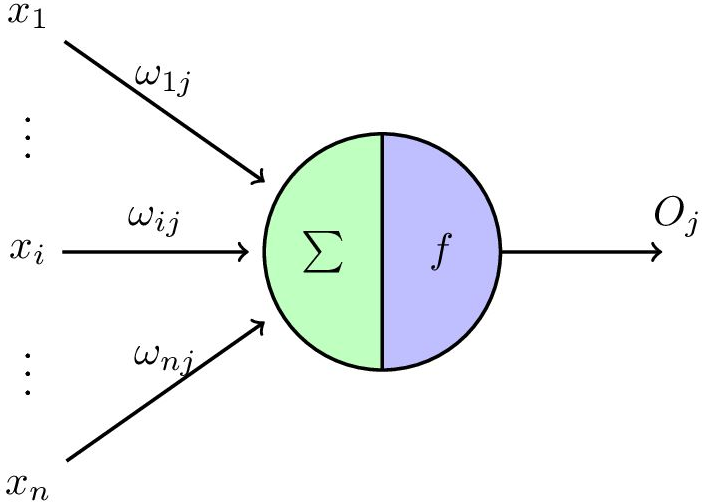
\includegraphics[scale=0.7]{Figures/mpmodel.png}
	\caption{M-P 模型}
\end{figure}
\begin{figure}
	\centering
	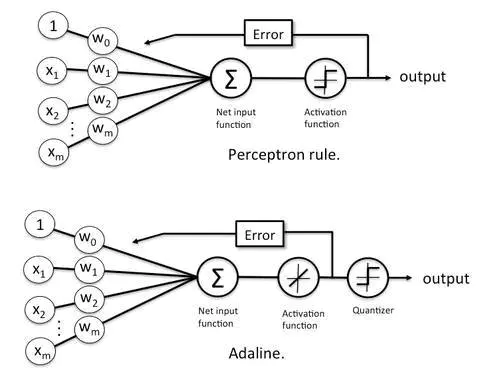
\includegraphics[scale=0.7]{Figures/perceptron.png}
	\caption{Perceptron 模型以及其改进模型 Adaline 网络}
\end{figure}

M-P 模型作为基于简单的函数运算和阈值逻辑来识别输入的二分类器人工神经网络,是最简单的人工神经网络的架构之一,首次在数学和计算模型领域引入仿生神经网络的思想,开辟了人工神经网络研究这个新的计算机科学领域.M-P模型的提出,证明仿神经网络的数学模型在一定程度上可以实现逻辑和算术函数映射的功能.而随后的一系列神经功能运行机制在数理上的抽象和在数学模型上的引入不断强化着人工神经网络模拟复杂映射能力.

而20世纪40年代末的 Donald Olding Hebb 通过在数学模型中引入对神经元的激活机制的抽象, 提出了用以调整其数学模型参数的 Hebb 学习规则, 以模拟神经元的选择性和差异性的激发来模拟生物神经元对外界刺激的学习机制. 1958年, Cornell 航空实验室的 Frank Rosenblatt 提出的模式识别算法感知机神经网络,即 Perceptron 神经网络,通过简单四则运算实现了结构简单的双层网络,并且数理化表述了感知机中尚无法实现的异或回路机制.Perceptron 神经网络引发了学界对神经网络结构和相关学习算法的广泛深入研究.其后, Stanford 大学教授 Bernard Widrow 和学生 Ted Hoff 也在 Perceptron 模型做出了基于 ALN ( Adaptive Linear Neuron , 适应性线性神经元)的 改进型的 Adaline 网络. Perceptron 模型和 Adaline 模型见图 1.2 .

但是上述的 M-P 模型与 Perceptron 模型及其改进型作为早期神经网络模型的代表,在 1969 年被 Marvin Minsky 和 Seymour Papert 证明其功能上的有限性,尤其是无法实现 Frank Rosenblatt 所提出的异或回路机制,这一度成为了该领域的研究瓶颈. 

随后, Paul Werbos 博士的误差反向传播机制,即 BP (Back-propagation,反向传播) 算法的提出,使得异或回路的实现在理论上出现了可能,但是在网络神经元结构上的限制使得 BP 算法仍难以得到有效利用.

最终 John Hopfield 与 Hinton, G. E. 和 Sejnowski, T. J. 在多层神经网络模型中,引入全互联机制和隐单元结构,使得神经网络领域再次进入蓬勃发展时期. 而 David E. Rumelhart, Geoffrey E. Hinton 和 Ronald J. Williams 提出的非线性 sigmod 函数神经元与误差反向传播算法即 BP 算法的结合,解决了异或回路问题.另外,1997年 Sepp Hochreiter 和 Jürgen Schmidhuber 提出根据对人类神经活动中记忆的遗忘机制,也进一步加强了人工神经网络在功能概念上的仿真程度.

像这样的大量的有效的对神经功能模块进行数理化仿真的功能单元的引入,并且使得相对复杂的非纯线性多层神经网络,成为人工神经网络结构的重要组成形式,使得人工神经网络的训练和广泛应用更具有可行性.

\section{人工神经网络发展和深度学习}
%见 许可_卷积神经网络在图像识别上的应用的研究 1.2节 引用[13][15]
%来自wikipedia
%百度百科 深度学习
深度学习作为机器学习的重要形式,其发展和人工神经网络的架构的发展也存在一定的同步性,两者都在一定的层面上存在对人工神经功能的模拟借鉴.

人工神经网络是在生物学研究的基础上,通过多学科交叉领域学界的的探索,最终衍生出的计算机科学研究领域.按照机器学习以及认知科学领域目前普遍认同的定义,人工神经网络是一种可以根据外部信息进行自适应的仿生数学或计算模型,这明显是对生物神经系统学习能力的数理化抽象和应用.

%此段引用[13][15]
而深度学习同样存在对生物神经机理的抽象.20世纪到如今不断发展的脑科学技术研究,除了在组织和细胞层面进行结构和功能分析,其在大脑各分区的功能判断也对人工智能技术发展有所助益.大脑新皮层感知能力的发现,成为其中典型的样例.

研究表明,大脑新皮层作为哺乳动物很多感知能力的物质基础,其结构上不依赖于对外部刺激的非结构化预处理,而是将时间上连续的外部刺激信息通过模型结构层次式传递处理.经过大量相关的实验,研究者发现在长时间针对视觉样本的特定训练下,训练目标能力的图像化边界不断地从粗糙变得精确化.

%[17]
此前,深度学习对在高维样本特征学习的过度困难无能为力,即 Richard Bellman 所称的的"维度灾难".但是神经结构感受能力在长时间训练中判别能力边界的不断精确化,给予了深度学习中的特征学习有意义的借鉴. 大脑性皮层对于与数据在感知模块中长时间的层次性传播对学习能力的实现,在某种程度上,同时依赖于对高维样本特征的降维,以及对时间意义上连续的样本特征之间上具有一定相似性的假设.

在此基础上,深度学习在人工神经网络中的体现,可以归纳为以样本处理的手段学习其中的某些复杂的分析特性与分布规律,使得样本在经过模型处理的过程中,不断使分布式数据特征精确化,而这些特征表达则是目标分析处理能力的数理化表述.

\section{全连接网络与卷积神经网络}
%https://blog.csdn.net/jinking01/article/details/103344186?spm=1001.2101.3001.6650.5&utm_medium=distribute.pc_relevant.none-task-blog-2%7Edefault%7EBlogCommendFromBaidu%7ERate-5.pc_relevant_paycolumn_v3&depth_1-utm_source=distribute.pc_relevant.none-task-blog-2%7Edefault%7EBlogCommendFromBaidu%7ERate-5.pc_relevant_paycolumn_v3&utm_relevant_index=8
基本的非纯线性多层神经网络,在研究的早期被认为在应用领域具有巨大的价值.而且在1989年,通过大量针对包含隐单元和非线性单元结构的多层神经网络中 BP 算法性能的探究,最终在理论上证明了在神经网络层数和隐藏层数足够的情况下,基本非纯线性多层连续前馈神经网络可以任意程度逼近任意的映射.

但是,实际上应用这种思想的全连接神经网络在实际训练和应用中效果并不理想.虽然理论上全连接神经网络能够拟合任意的映射,但实际上过度复杂的神经网络结构会造成得到目标分析处理能力和参数良性收敛的失败,使得基于海量数据集的有效深度学习变得困难.因此,为增强人工神经网络在深度学习训练上的易行性,必须在其数理结构上复杂性和实际应用上的有效性中做出取舍.

在1979年,日本工程师 Kunihiko Fukushima 提出 Neocognitron 网络,并在其中引入了"卷积"和"池化"等不包含在传统非纯线性多层神经网络中的功能概念,这使得神经网络在组织结构上出现进一步的复杂化.1989年 Yann LeCun 提出的 LeNet 神经网络成为以一个系统化实现相关性概念的卷积神经网络.通过对基本非纯线性多层神经网络的针对性改进而产生的卷积神经网络,具有与传统的全连接网络不同的神经网络架构,很好的解决了全连接网络在实际应用中一部分缺陷.

\begin{figure}
\centering
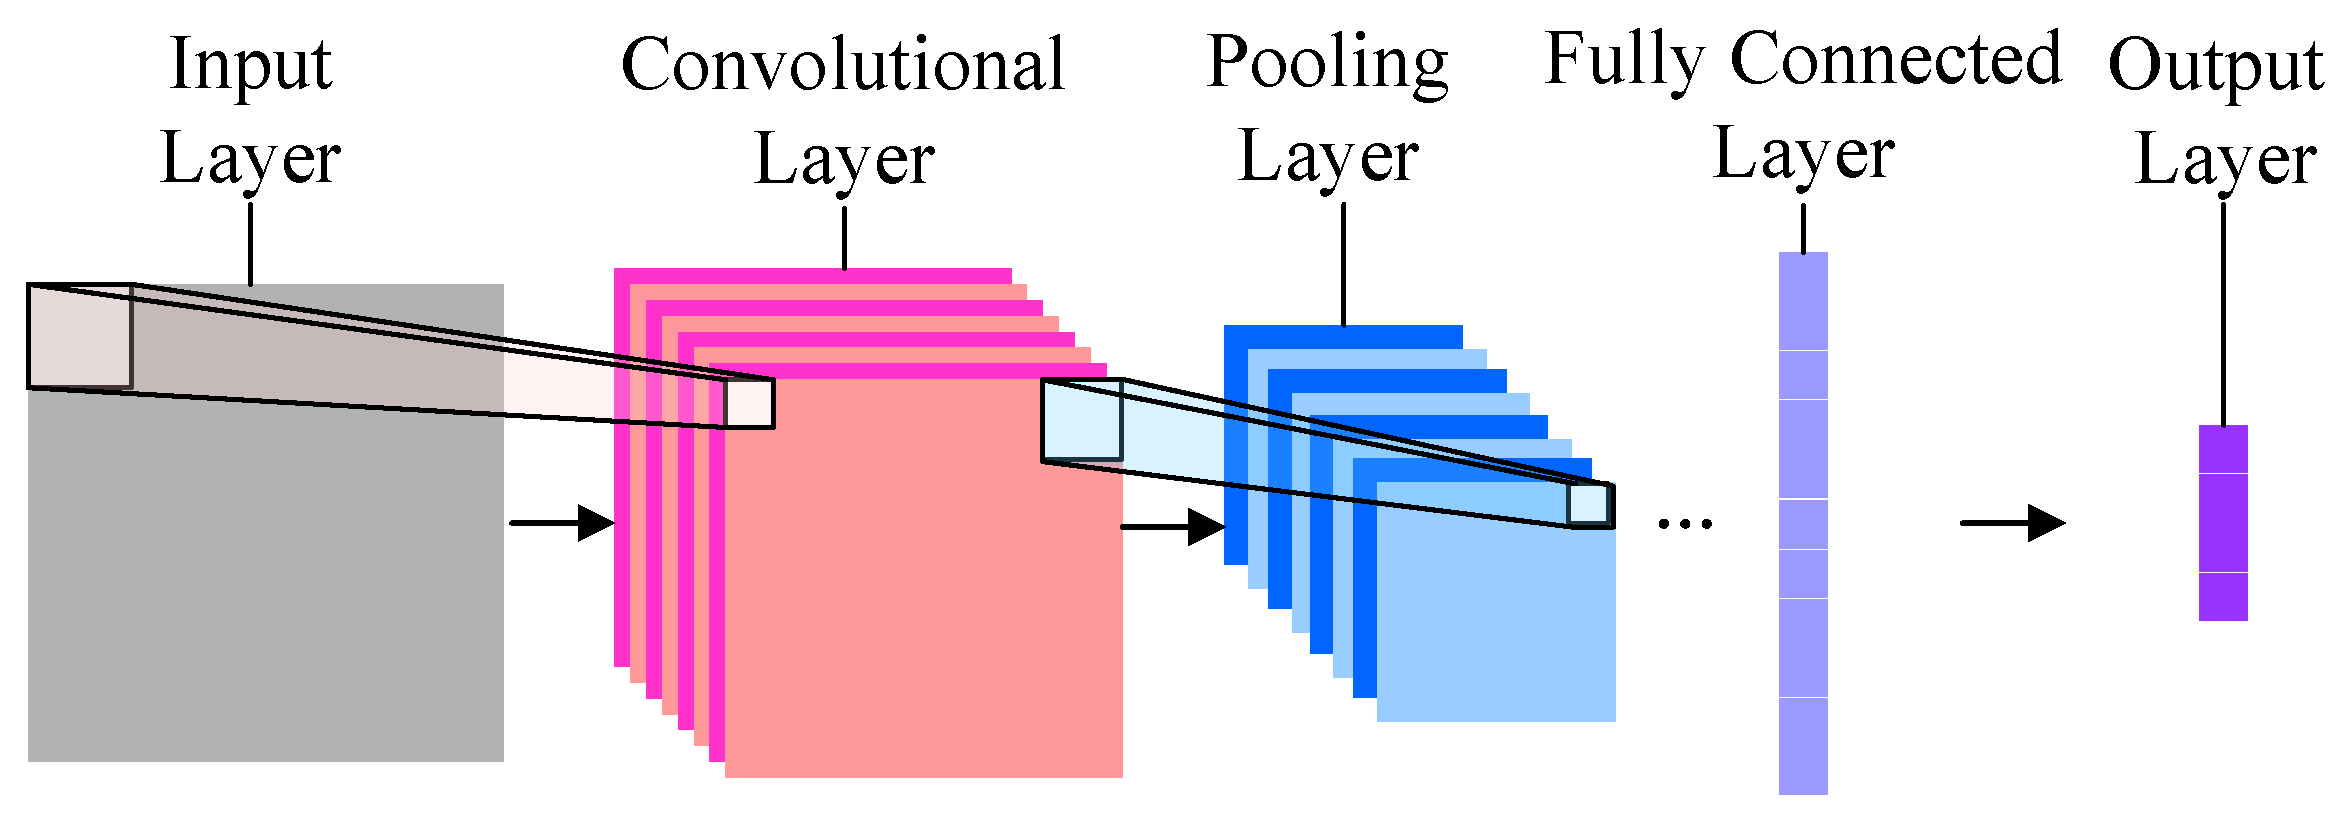
\includegraphics[scale=1]{Figures/CNN3.png}
\caption{卷积神经网络结构}
\end{figure}

这是因为,在卷积神经网络在传统的全连接神经网络结构之外,还引入了以下的结构:
\begin{enumerate}
	\item 激活层 RELU : 应用非线性激励函数的非线性层,具有对线性映射性能不足进行补充,并使输出控制在一定范围内的功能,作为卷积层和输出层的一部分
	\item 池化层 POOLING : 具有在不同深度上欠采样,降低特征的维度,防止过拟合的功能
	\item 输入层 INPUT : 预处理多维输入,具有将将输入数据去均值和归一化,再在各个维度上降维形成若干不相关的特征轴功能的神经元层
	\item 卷积层 CONV : 一种基于在各神经元多维感受域下的局部感知效应的而实现参数共用的复杂计算单元层
	\item 输出层 OUTPUT : 神经网络的最后一层,由线性层和具有概率分布映射功能的$softmax$函数组成,视为多分类器
\end{enumerate}

典型卷积神经网络的基本结构见图 1.3 .

在这些新的结构中,输入层实现了复杂多维数据在进入网络前的规范化处理,复数的卷积层的并用能够更加充分的利用输入的多维特征,而池化层的欠采样功能则能够抛弃多余的多维特征并在一定程度上避免过拟合的情况,而输出层作为标签预测模型的重要构件具有求取各目标标签概率分布的功能.

而总体上来说,由于卷积神经网络存在模型参数共用和多维特征采集的机制,导致实际上模型的参数量更精简.由于卷积神经网络在模型权重参数上的有效精简,使得其无论是在深度学习训练难度还是实际使用场景中的有效性都更高.

\section{卷积神经网络与图像识别}
%来自
%https://zhuanlan.zhihu.com/p/47184529?msclkid=506087dbb97811ec8040aa32dc937a8c

神经网络在图像识别领域的应用,是推动人工神经研究领域进步的现实动力之一.在诸多的人工神经网络模型概念中,卷积神经网络是最有应用价值和研究价值的领域之一.卷积神经元相比全连接的人工神经网络,更加具有广泛应用的潜力.

1998年, Yann LeCun 与其他共同研究者在自己提出的 LeNet 卷积神经网络模型的基础上提出了改进的 CNN LeNet-5 人工神经网络用以对美国的支票等文书上的手写数字进行精确识别.

这种人工神经网络在社会经济领域的直接应用,极大地促进了人工智能领域学界对神经网络实际运行性能追求和相关算法和结构的改进,并使得标准化的人工神经网络图像识别成为衡量神经网络性能的重要指标之一.卷积神经网络相对于全连接的神经网络,能够有效避免全连接网络对多维输入向量化造成的信息损失,同时也避免了实际应用中全连接网络中大量的冗余参数造成训练困难和过拟合现象.

因此,在图像识别领域的应用上,卷积神经网络的确相对其他更原始形式的人工神经网络更加具有竞争力和实用性.

LeNet 卷积神经网络在 MNIST 手写数据集上的应用见图 1.4 .

\begin{figure}
	\centering
	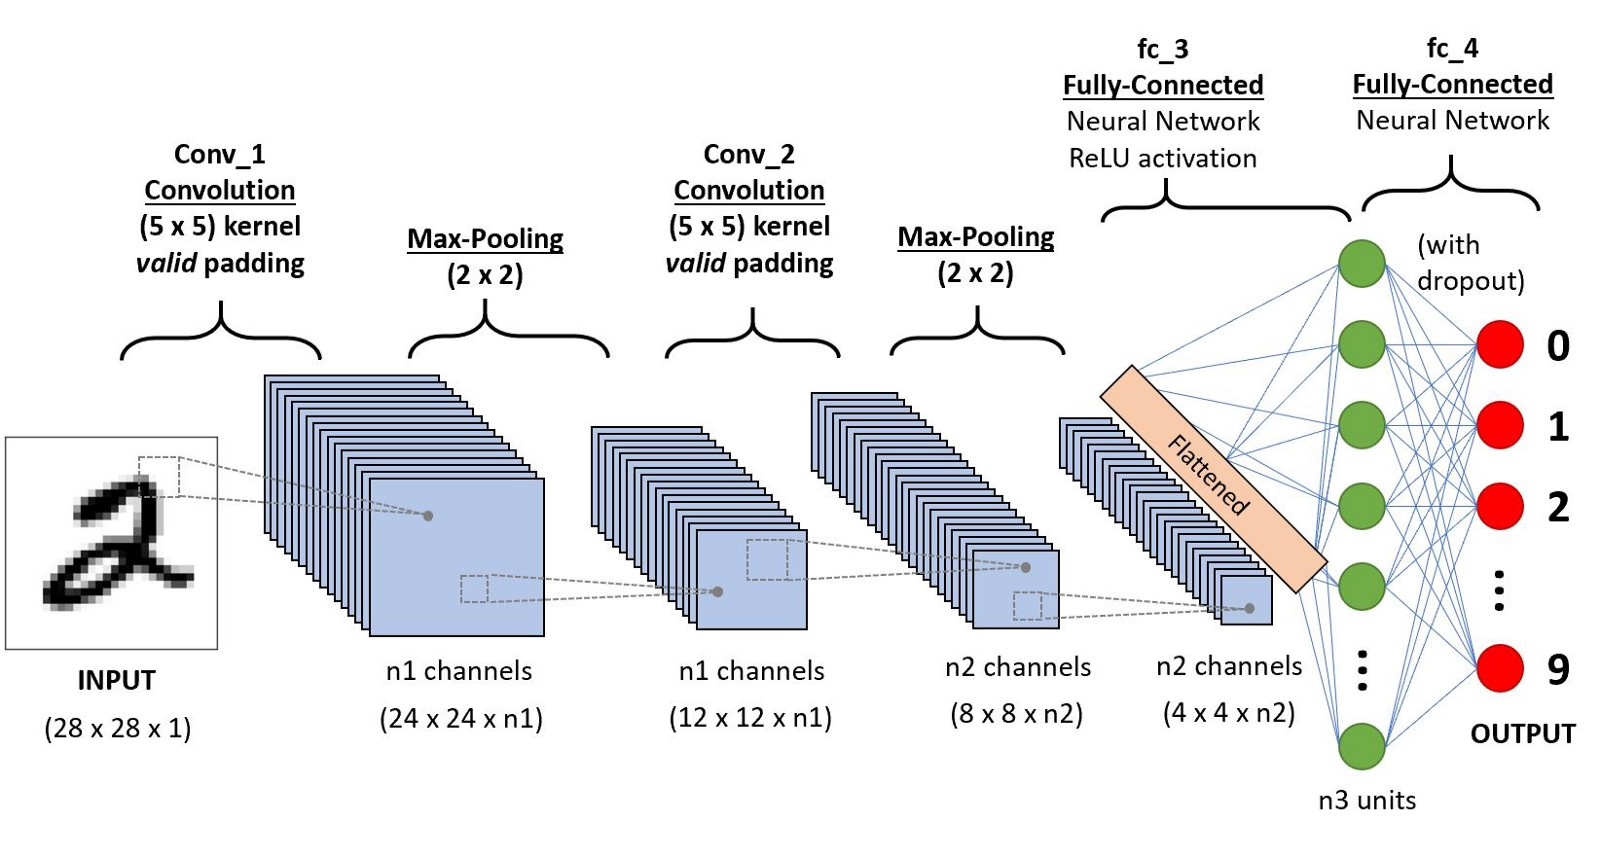
\includegraphics[scale=0.2]{Figures/CNN2.jpg}
	\caption{卷积神经网络在图像识别上的应用}
\end{figure}

\chapter{神经网络应用的安全问题}

因为人工神经网络技术在社会各领域的广泛运用,使得人工神经网络的应用项目本身变成了具有重大政治、经济乃至文化价值的影响目标.因此,围绕人工神经网络在应用上的安全性,对相关攻击手段和防御方式开始变得越来越被重视.

\section{神经网络安全问题的常见场景}
% 见我的相关md文档,引用来自Backdoor Learning: A Survey Yiming Li, Baoyuan Wu, Yong Jiang, Zhifeng Li, and Shu-Tao Xia

\begin{figure}
	\centering
	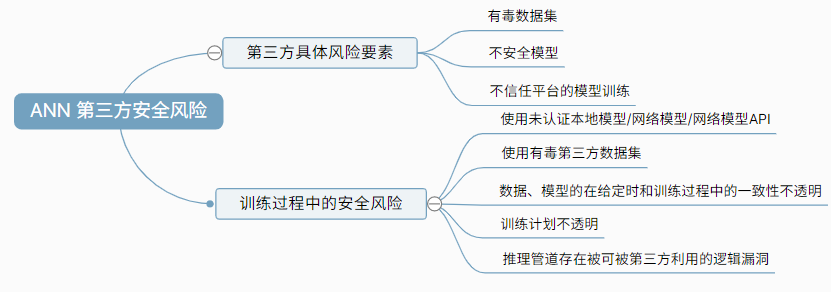
\includegraphics[scale=0.7]{Figures/situation.png}
	\caption{人工神经网络应用中的风险}
\end{figure}

目前,围绕人工神经网络实际应用的各类攻击手段并不统一.若不在应用场景中没有第三方情形下考虑安全问题的话,则可以通过第三方在人工神经网络应用场景中的不同参与方式,来区分不同类别安全风险的特点.现代社会的人工神经网络应用中,第三方的人工神经网络计算平台以及第三方的数据集和模型,都是潜在的第三方参与的有安全隐患的应用场景.

根据这些这些常见的风险形式,我们可以划分出第三方平台、第三方数据、第三方模型三个主要场景.

在第三方平台控制下进行训练,存在模型和数据被篡改的风险.虽然第三方平台可能实现对运行参数的透明,但仍然不能排除训练过程中暗中修改模型或训练过程计划,以及修改用户方提供的良性数据集插入有毒数据等恶意行为的存在.对这样的场景尚没有能完全消除恶意风险的手段,一般可以通过在良性环境下重复训练以调整恶意修改模型造成的效果.

在可能恶意的第三方数据集的影响下,除了通过某些方式清除有毒数据外也没有根本的解决方式.但是这种情形下的安全风险仅限于有毒数据,而无法对模型结构、训练过程计划、推理管道造成影响.

有恶意风险的第三方模型,一般在应用场景中通过互联网和源码非透明公开的 API 引入.这类型的安全风险在几类场景中是最大的,因为有毒的模型可以污染模型无关的推理管道外几乎所有的处理过程.针对这种安全风险,需要在人工神经网络输入数据的预处理阶段或是推理管道的功能上做出有效的防范.

\section{针对人工神经网络的常见攻击与防御分析手段}
\subsection{常见的攻击手段}
%见我的相关md文档
%见https://www.anquanke.com/post/id/255550
除了针对人工神经网络的攻击手段不统一之外,攻击所期望达成的形式和目的同样具有差异性.按照类似于计算机病毒威胁的划分,我们可以将针对神经网络的攻击划分为非指向性的功能失效与有指向性和目的性的功能变化诱导.

功能失效的主要体现是人工神经网络功能的普遍降低或失效,在常见的分类器神经网络模型上,具体表现可以是对各类测试样本分析有效率的全面降低.在这方面典型的攻击手段是第三方的普遍数据投毒,因为普遍数据投毒会造成神经网络决策边界错误转移和混淆.

而功能变化诱导则是需要藉由攻击,影响人工神经网络实现新的特定功能,一般不会对网络功能做出彻底破坏.在这方面的典型手段则是后门植入,也是本文所关注的重要攻击手段.后门植入可以在分类器上实现对特定类指向性的分析功能破坏.


\begin{figure}
	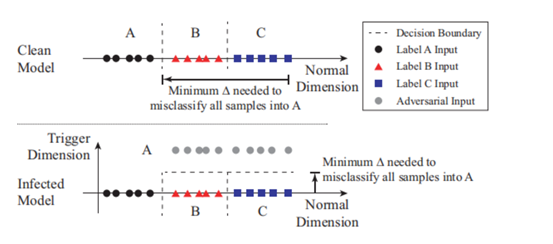
\includegraphics[scale=0.5]{Figures/toudu.png}
	\caption{数据投毒对多分类器决策边界转移的表现}
\end{figure}
\begin{figure}
	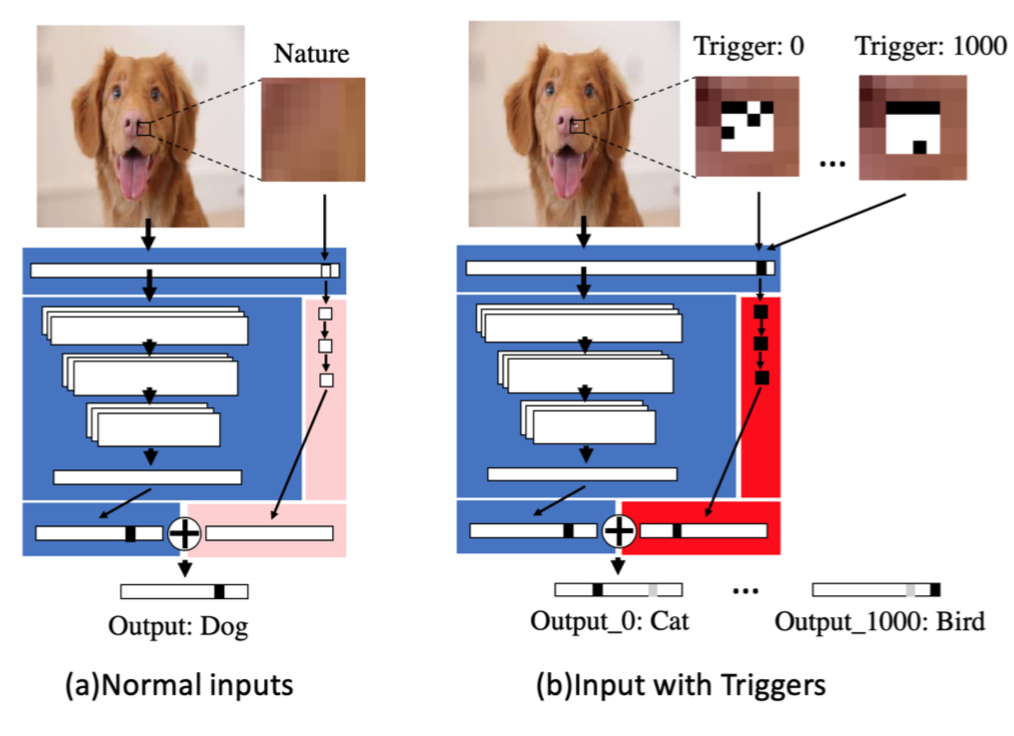
\includegraphics[scale=0.5]{Figures/houmen.png}
	\caption{多分类器上后门的运行原理}
\end{figure}
\subsection{具体的先进防御分析手段}

近些年来,人工神经网络的攻击技术的发展促使着防御分析技术同步发展,以 NC 法 , AC 法, SentiNet 法 , STRIP 法为代表的等多种防御分析手段体现了重要的研究价值.如下我们对这些防御分析方法进行原理和运用上的分析.
\begin{enumerate}
	%\begin{figure}
	%	\includegraphics[scale=0.5]{Figures/.png}
	%	\caption{多分类器上后门的运行原理}
	%\end{figure}
	%没想好插什么图
	
	%[针对后门攻击的防御手段之Neural Cleanse](https://www.jianshu.com/p/ffe1c966faee)
	
	%参考论文Demon in the Variant: Statistical Analysis of DNNs for Robust Backdoor Contamination Detection 的[42]号引用
	\item NC 法( Neural Cleanse ,神经清理):一类基于分类特征抽象分解的针对后门植入的防御手段.
	
	若将样本的特征区分抽象视为在模型分类维度上的区分和后门触发器维度上的区分的复合,那么此类防御基于两个假设.假设一,带后门的模型对应的触发器比正常模型形成的触发器相关决策边界更小.假设二,在感染模型中能引起误分类的沿触发器方向的最小变化量小于正常模型.
	
	后门分析过程中,需要通过反向构造将输入预处理为有相关系数的带触发器的输入,并通过这些带触发器的输入求取结果的 L1 范数来判断触发器的大小.当对应的异常指标过大时则认定需要神经清理.在清理过程中,根据神经元的激活值选择性裁剪神经元,移除激活值畸高的节点分支.
	
	这种防御方式同时具有具体性能和理论上的缺陷.是有效的清理过程虽会大幅攻击成功率,但同时会小幅降低对良性样本的分析准确度.而理论上,神经清理无法也捕获不依赖优势属性的潜在触发器.
	
	%参考论文Demon in the Variant: Statistical Analysis of DNNs for Robust Backdoor Contamination Detection 的[4]号引用
	\item AC 法( Activactive Cluster ,聚类激活分析法):一类基于神经元激活情况在降维聚类分析后特征的分析手段.
	
	若将后门样本识别为指定类的过程,视为污染特征对高优先级指定类触发器的触发以及源类特征对正确分类的触发的叠加.那么由于正常样本不存在对触发器的触发,两类样本在神经网络中的神经元激活状态也不同.
	
	在操作上,分析目标数据集在经过神经网络处理过程中神经元的激活情况分布,需要使用降维和聚类的手段,将神经网络最后一层输出降维聚类得到分布图.
	
	目标分布图是二维平面上的点的集合,划分为若干个集中区域称为簇.一般中毒样本所集中的簇规模相对较小,而代表正常样本的各个簇的规模往往接近.当出现规模显然过小的簇时,一般可以认定数据集合模型受到了污染.
	
	%SentiNet总结_遠い世界へ-CSDN博客](https://blog.csdn.net/weixin_42561013/article/details/120579016
	%参考论文Demon in the Variant: Statistical Analysis of DNNs for Robust Backdoor Contamination Detection 的[8]号引用
	\item SentiNet 法:一类基于图像多分类器的触发器的触发区域限制的分析手段. SentiNet 法的不仅可以对模型的后门进行分析,还可以分析甚至定位触发器所在的区域.
	
	所谓的 SentiNet 分析法,需要选定建议类、划分掩盖区域、选定区域遮掩方式.其中选定的特定建议类作为遮掩行为调整的对象,遮掩行为则是通过惰性触发器使得特定建议类的分类能力.而划分掩盖的区域,则是在图像中选取触发器可能候选的若干相关区域.由于触发器所在的候选区域的输入一般在卷积网络运行时较为重要和活跃,因此 Grad-CAM 热力图算法等手段可以筛选出这些高重要度区域.
	
	在分析时,需要在并行的测试中各选定不同的单一建议类,确定各种建议类下的分类结果的平均置信度和称为愚弄计数的错误分类数并绘制为二维点图.而测试的输入需要随机噪声和选定污染样本作为对照,因为两者在二维点图上的拟合特性明显不同.随机噪声的二维点图一般可以拟合为直线,而污染样本在图像上的样本点则一般同时具有高愚弄计数和低置信度.
	
	%STRIP: A Defence Against Trojan Attacks on Deep Neural Networks ,https://blog.csdn.net/Billy1900/article/details/120084537
	\item STRIP 法:一类基于熵分析的对后门植入的分析手段,这类方法假设带触发器或受污染的输入的结果熵较低.
	
	在操作中, STRIP 法的后门分析,基于对任一自然被污染的输入进行特定方式均匀混淆处理而衍生的系列扰乱输入,在通过带触发器的模型后,其结果相对低熵的假设.
	
	但这种防御方式虽然可以同时对样本输入和模型本身特性进行分析,但对未被植入后门的模型无效,也同时可能会因为扰乱输入对触发器的误触发导致熵畸高.
	 
\end{enumerate}

%引用来自Demon in the Variant: Statistical Analysis of DNNs for Robust Backdoor Contamination Detection /Di, Tang
2021年,在 Di Tang 等人针对后门污染分析的论文研究中,指出了如上的几类防御分析手段缺乏对样本特征的统计化和解析化分析手段的缺点,提出了统计污染分析法即 SCAn 法.SCAn 法对样本特征的处理手段相对更加注重统计特性.

SCAn 法将样本特征向量化,并进行双成分分解,分解为代表分类特性的恒常分量和服从高维特定分布的变异分量之和.先使用良性样本集,通过数学统计手段,估计恒常分量与变异分量分布参数的值.在判断任一不确定样本集时,将高维分布的参数参考值带入分布类型进行假设检验,判断参数向量的置信度是否符合假设,若良性样本集假设不成立,则表明给定样本是非良性样本集.

由此可见,SCAn 法相对上述其他诸主流方法,更加依赖统计特性,具有更高的细粒度.因此, SCAn 法能够更加精确的区分有毒样本和一般样本,甚至可以针对不典型的、不规律的分布方式的触发器进行捕获,在应用上具有相当高的普遍性.

\section{本文的观点}

上述的诸多主流的人工神经网络防御分析手段,在分析所依靠的假设理论上都有可借鉴的方面.首先, SCAn 法的双成分分解法,表明对良性样本集和污染样本集可以依赖统计特征的区分.而 STRIP 法对人工神经网络输出结果的熵分析,一定程度上也可作借鉴,甚至可以推广到模型间的层级上.

在一定程度上,由于有效神经网络训练规模的庞大性与结构的复杂性,学界目前对人工神经网络内部权重参数分布特征与神经网络后门间的对应关系仍不能充分解析,因此本文选择绕开对神经网络本身内部特性的探究,选择从恶意样本与神经网络后门对神经网络的输出特性的影响进行研究.

为充分研究神经网络的输出特性,需要从大量神经网络的输出中得到分布的输出规律.本文意图通过在不同数据下进行差异化训练的同质的卷积神经网络模型在测试集中对特定对象进行分布式的预测,并通过比较不同模型间的预测差异,来从目标测试集中提取某些特定样本相对于良性样本的异常特性.

\chapter{卷积神经网络的投票式模型}

\section{MNIST数据集的使用}

MNIST数据集作为在卷积神经网络中被广泛使用的数据集

\section{卷积神经网络的选取}

本次实验选取的是在图像识别领域常用的 LeNet 卷积网络模型
%% -*- coding: GBK2312 -*-

%\chapter{绪论} \label{chpt:A}

\chapter{绪论}

%来自wikipedia
%百度百科 深度学习
人工智能技术,本质上是寻求以某种形式和程度上的自动化,以求在特定方面替代在各种生产与生活领域对人力资源以及人力控制的需求.其作为目前国际学界最为关注的研究领域之一,其对社会发展的影响力和推动力难以估量.

而人工智能技术所需要的具有应用价值的人工智能系统,必须能够在一定程度上模拟人的控制能力.而模拟人的控制能力,在理论上需要机器学习的手段和载体以及对相关能力特征的表述. 而ANN ( artificial neural network ,人工神经网络)与深度学习,正是被广泛运用的人工智能的载体与学习手段.

在计算机科学领域,由于在大量人工智能需求场景下都具有的通用性和有效性,使得如今在计算机识别和控制、统计规划、医学以及生物研究乃至社会经济等领域, ANN 和深度学习技术都是最具价值的研究方向之一.

\section{人工神经网络与神经活动研究}

%以下内容来自
%https://blog.csdn.net/jinking01/article/details/103344186?spm=1001.2101.3001.6650.5&utm_medium=distribute.pc_relevant.none-task-blog-2%7Edefault%7EBlogCommendFromBaidu%7ERate-5.pc_relevant_paycolumn_v3&depth_1-utm_source=distribute.pc_relevant.none-task-blog-2%7Edefault%7EBlogCommendFromBaidu%7ERate-5.pc_relevant_paycolumn_v3&utm_relevant_index=8

%来自https://www.zhihu.com/question/54139566 Frankenstein的回答

人工神经网络技术领域具有很深刻的多学科领域交叉的历史背景,可以追溯到医学和生物研究领域对人类神经活动的研究模拟. 而正是对神经系统和神经结构特性的不断模拟和数理化抽象,促进着人工神经网络形式和功能上的不断复杂化和精确化,这是一个不断进步的过程.

奥地利医生 Franz Joseph Gall 通过对人类神经组织切片的微观分析,得出了人类神经活动依赖于人体脑部的功能的论断,解释了人类神经功能的物质基础.在一定程度,这与神经网络所需求的分析能力,某种程度上依赖于人工神经网络的数理模型结构,逻辑关系上十分相似.

意大利细胞学家 Camillo Golgi 与西班牙神经组织学家 Santiago Ramón y Cajal 通过使用 Golgi 染色法等更精细的微观分析手段,确认了人类神经组织中神经元功能和结构的独立性.而神经元结构与功能上的独立性的科学发现,也为此后人工神经网络中仿神经元的计算单元设计提供了借鉴.

最终在1943年,基于 Franz Joseph Gall , Camillo Golgi 和 Santiago Ramón y Cajal 对人类神经功能运行模式的一系列深入研究, Warren McCulloch 和 Walter Pitts 首次提出借鉴已知神经细胞运行机制的数学模型 M-P 模型. M-P 模型见图 1.1 .

\begin{figure}
	\centering
	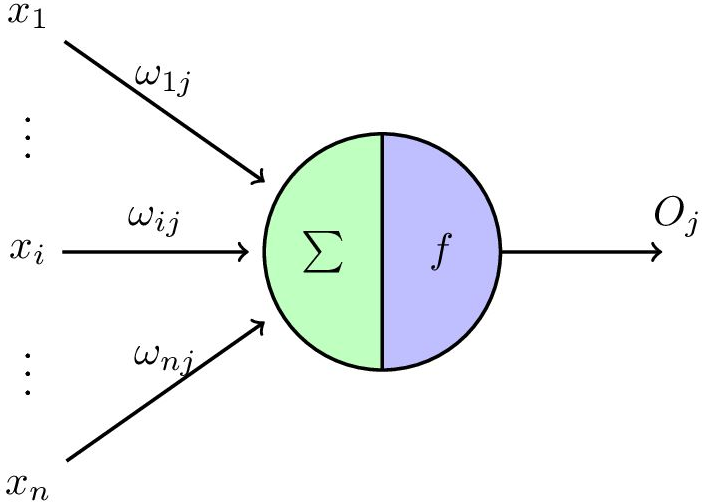
\includegraphics[scale=0.7]{Figures/mpmodel.png}
	\caption{M-P 模型}
\end{figure}
\begin{figure}
	\centering
	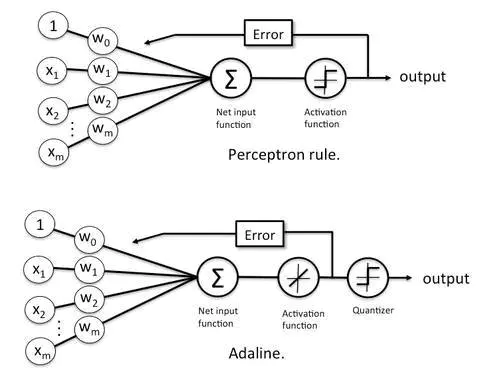
\includegraphics[scale=0.7]{Figures/perceptron.png}
	\caption{Perceptron 模型以及其改进模型 Adaline 网络}
\end{figure}

M-P 模型作为基于简单的函数运算和阈值逻辑来识别输入的二分类器人工神经网络,是最简单的人工神经网络的架构之一,首次在数学和计算模型领域引入仿生神经网络的思想,开辟了人工神经网络研究这个新的计算机科学领域.M-P模型的提出,证明仿神经网络的数学模型在一定程度上可以实现逻辑和算术函数映射的功能.而随后的一系列神经功能运行机制在数理上的抽象和在数学模型上的引入不断强化着人工神经网络模拟复杂映射能力.

而20世纪40年代末的 Donald Olding Hebb 通过在数学模型中引入对神经元的激活机制的抽象, 提出了用以调整其数学模型参数的 Hebb 学习规则, 以模拟神经元的选择性和差异性的激发来模拟生物神经元对外界刺激的学习机制. 1958年, Cornell 航空实验室的 Frank Rosenblatt 提出的模式识别算法感知机神经网络,即 Perceptron 神经网络,通过简单四则运算实现了结构简单的双层网络,并且数理化表述了感知机中尚无法实现的异或回路机制.Perceptron 神经网络引发了学界对神经网络结构和相关学习算法的广泛深入研究.其后, Stanford 大学教授 Bernard Widrow 和学生 Ted Hoff 也在 Perceptron 模型做出了基于 ALN ( Adaptive Linear Neuron , 适应性线性神经元)的 改进型的 Adaline 网络. Perceptron 模型和 Adaline 模型见图 1.2 .

但是上述的 M-P 模型与 Perceptron 模型及其改进型作为早期神经网络模型的代表,在 1969 年被 Marvin Minsky 和 Seymour Papert 证明其功能上的有限性,尤其是无法实现 Frank Rosenblatt 所提出的异或回路机制,这一度成为了该领域的研究瓶颈. 

随后, Paul Werbos 博士的误差反向传播机制,即 BP (Back-propagation,反向传播) 算法的提出,使得异或回路的实现在理论上出现了可能,但是在网络神经元结构上的限制使得 BP 算法仍难以得到有效利用.

最终 John Hopfield 与 Hinton, G. E. 和 Sejnowski, T. J. 在多层神经网络模型中,引入全互联机制和隐单元结构,使得神经网络领域再次进入蓬勃发展时期. 而 David E. Rumelhart, Geoffrey E. Hinton 和 Ronald J. Williams 提出的非线性 sigmod 函数神经元与误差反向传播算法即 BP 算法的结合,解决了异或回路问题.另外,1997年 Sepp Hochreiter 和 Jürgen Schmidhuber 提出根据对人类神经活动中记忆的遗忘机制,也进一步加强了人工神经网络在功能概念上的仿真程度.

像这样的大量的有效的对神经功能模块进行数理化仿真的功能单元的引入,并且使得相对复杂的非纯线性多层神经网络,成为人工神经网络结构的重要组成形式,使得人工神经网络的训练和广泛应用更具有可行性.

\section{人工神经网络发展和深度学习}
%见 许可_卷积神经网络在图像识别上的应用的研究 1.2节 引用[13][15]
%来自wikipedia
%百度百科 深度学习
深度学习作为机器学习的重要形式,其发展和人工神经网络的架构的发展也存在一定的同步性,两者都在一定的层面上存在对人工神经功能的模拟借鉴.

人工神经网络是在生物学研究的基础上,通过多学科交叉领域学界的的探索,最终衍生出的计算机科学研究领域.按照机器学习以及认知科学领域目前普遍认同的定义,人工神经网络是一种可以根据外部信息进行自适应的仿生数学或计算模型,这明显是对生物神经系统学习能力的数理化抽象和应用.

%此段引用[13][15]
而深度学习同样存在对生物神经机理的抽象.20世纪到如今不断发展的脑科学技术研究,除了在组织和细胞层面进行结构和功能分析,其在大脑各分区的功能判断也对人工智能技术发展有所助益.大脑新皮层感知能力的发现,成为其中典型的样例.

研究表明,大脑新皮层作为哺乳动物很多感知能力的物质基础,其结构上不依赖于对外部刺激的非结构化预处理,而是将时间上连续的外部刺激信息通过模型结构层次式传递处理.经过大量相关的实验,研究者发现在长时间针对视觉样本的特定训练下,训练目标能力的图像化边界不断地从粗糙变得精确化.

%[17]
此前,深度学习对在高维样本特征学习的过度困难无能为力,即 Richard Bellman 所称的的"维度灾难".但是神经结构感受能力在长时间训练中判别能力边界的不断精确化,给予了深度学习中的特征学习有意义的借鉴. 大脑性皮层对于与数据在感知模块中长时间的层次性传播对学习能力的实现,在某种程度上,同时依赖于对高维样本特征的降维,以及对时间意义上连续的样本特征之间上具有一定相似性的假设.

在此基础上,深度学习在人工神经网络中的体现,可以归纳为以样本处理的手段学习其中的某些复杂的分析特性与分布规律,使得样本在经过模型处理的过程中,不断使分布式数据特征精确化,而这些特征表达则是目标分析处理能力的数理化表述.

\section{全连接网络与卷积神经网络}
%https://blog.csdn.net/jinking01/article/details/103344186?spm=1001.2101.3001.6650.5&utm_medium=distribute.pc_relevant.none-task-blog-2%7Edefault%7EBlogCommendFromBaidu%7ERate-5.pc_relevant_paycolumn_v3&depth_1-utm_source=distribute.pc_relevant.none-task-blog-2%7Edefault%7EBlogCommendFromBaidu%7ERate-5.pc_relevant_paycolumn_v3&utm_relevant_index=8
基本的非纯线性多层神经网络,在研究的早期被认为在应用领域具有巨大的价值.而且在1989年,通过大量针对包含隐单元和非线性单元结构的多层神经网络中 BP 算法性能的探究,最终在理论上证明了在神经网络层数和隐藏层数足够的情况下,基本非纯线性多层连续前馈神经网络可以任意程度逼近任意的映射.

但是,实际上应用这种思想的全连接神经网络在实际训练和应用中效果并不理想.虽然理论上全连接神经网络能够拟合任意的映射,但实际上过度复杂的神经网络结构会造成得到目标分析处理能力和参数良性收敛的失败,使得基于海量数据集的有效深度学习变得困难.因此,为增强人工神经网络在深度学习训练上的易行性,必须在其数理结构上复杂性和实际应用上的有效性中做出取舍.

在1979年,日本工程师 Kunihiko Fukushima 提出 Neocognitron 网络,并在其中引入了"卷积"和"池化"等不包含在传统非纯线性多层神经网络中的功能概念,这使得神经网络在组织结构上出现进一步的复杂化.1989年 Yann LeCun 提出的 LeNet 神经网络成为以一个系统化实现相关性概念的卷积神经网络.通过对基本非纯线性多层神经网络的针对性改进而产生的卷积神经网络,具有与传统的全连接网络不同的神经网络架构,很好的解决了全连接网络在实际应用中一部分缺陷.

\begin{figure}
\centering
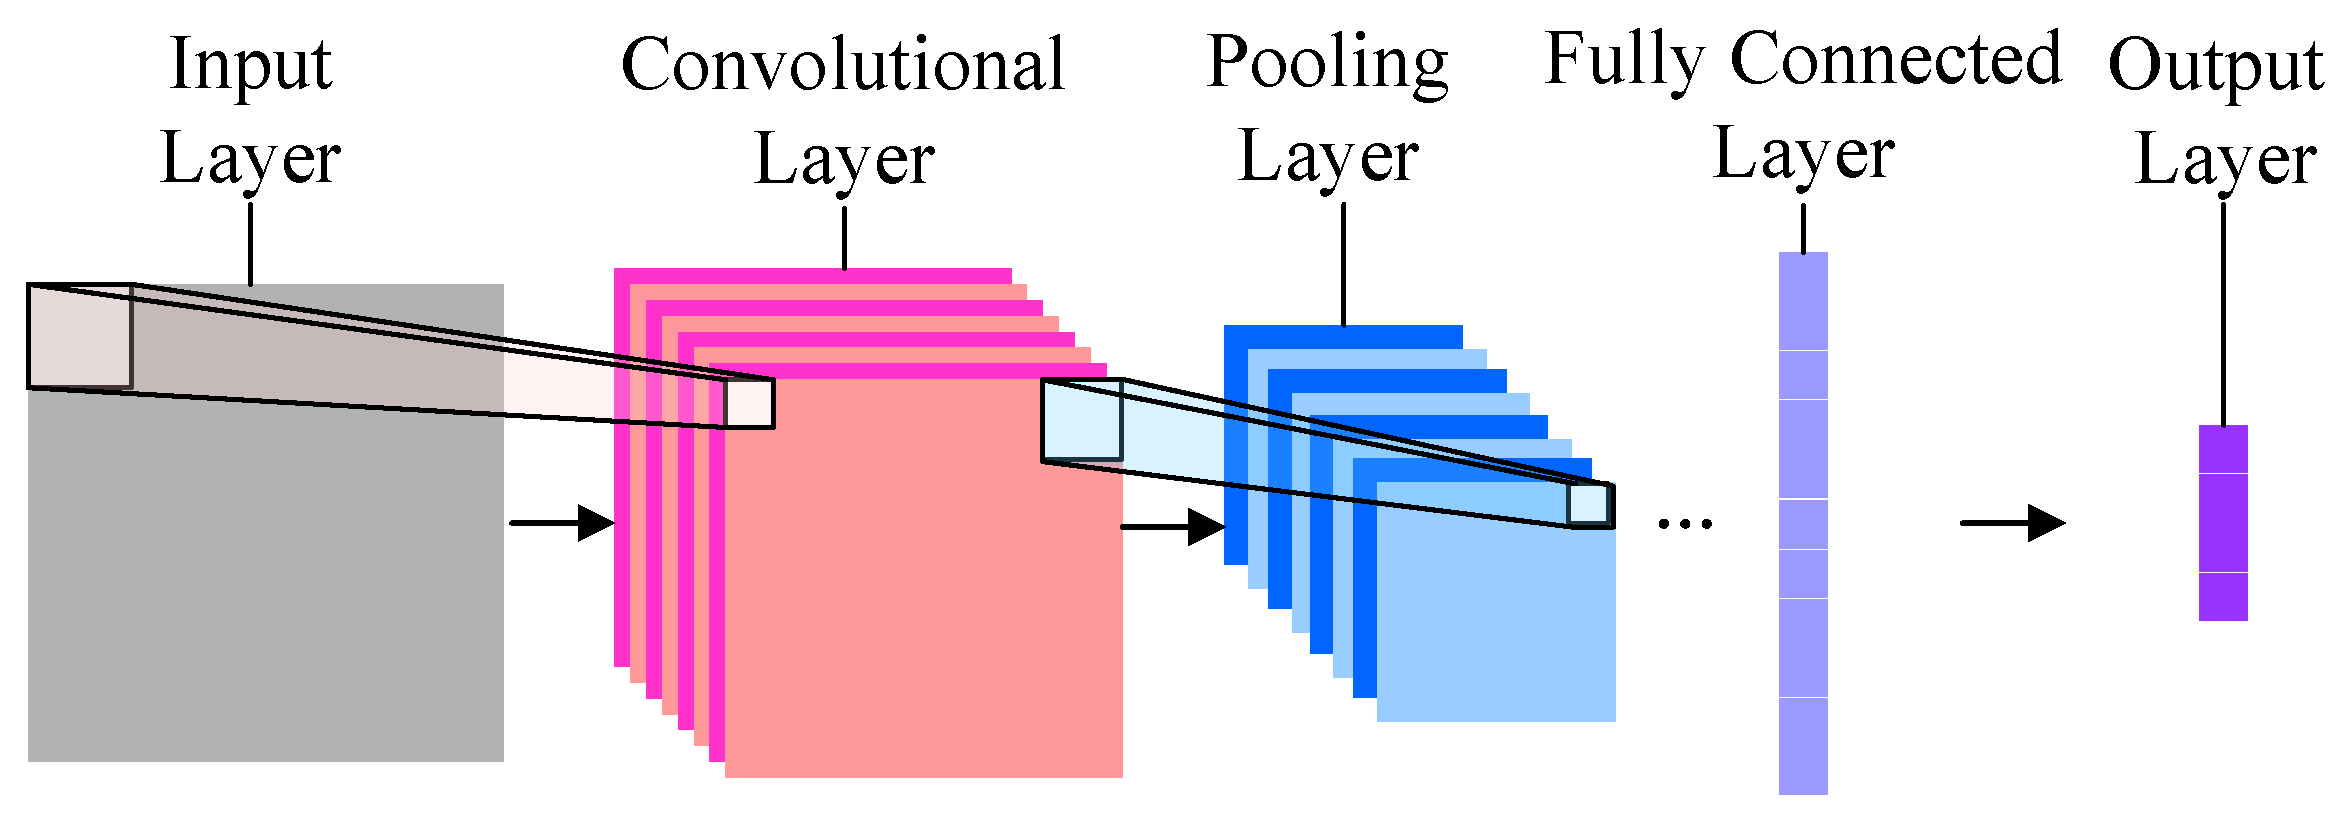
\includegraphics[scale=1]{Figures/CNN3.png}
\caption{卷积神经网络结构}
\end{figure}

这是因为,在卷积神经网络在传统的全连接神经网络结构之外,还引入了以下的结构:
\begin{enumerate}
	\item 激活层 RELU : 应用非线性激励函数的非线性层,具有对线性映射性能不足进行补充,并使输出控制在一定范围内的功能,作为卷积层和输出层的一部分
	\item 池化层 POOLING : 具有在不同深度上欠采样,降低特征的维度,防止过拟合的功能
	\item 输入层 INPUT : 预处理多维输入,具有将将输入数据去均值和归一化,再在各个维度上降维形成若干不相关的特征轴功能的神经元层
	\item 卷积层 CONV : 一种基于在各神经元多维感受域下的局部感知效应的而实现参数共用的复杂计算单元层
	\item 输出层 OUTPUT : 神经网络的最后一层,由线性层和具有概率分布映射功能的$softmax$函数组成,视为多分类器
\end{enumerate}

典型卷积神经网络的基本结构见图 1.3 .

在这些新的结构中,输入层实现了复杂多维数据在进入网络前的规范化处理,复数的卷积层的并用能够更加充分的利用输入的多维特征,而池化层的欠采样功能则能够抛弃多余的多维特征并在一定程度上避免过拟合的情况,而输出层作为标签预测模型的重要构件具有求取各目标标签概率分布的功能.

而总体上来说,由于卷积神经网络存在模型参数共用和多维特征采集的机制,导致实际上模型的参数量更精简.由于卷积神经网络在模型权重参数上的有效精简,使得其无论是在深度学习训练难度还是实际使用场景中的有效性都更高.

\section{卷积神经网络与图像识别}
%来自
%https://zhuanlan.zhihu.com/p/47184529?msclkid=506087dbb97811ec8040aa32dc937a8c

神经网络在图像识别领域的应用,是推动人工神经研究领域进步的现实动力之一.在诸多的人工神经网络模型概念中,卷积神经网络是最有应用价值和研究价值的领域之一.卷积神经元相比全连接的人工神经网络,更加具有广泛应用的潜力.

1998年, Yann LeCun 与其他共同研究者在自己提出的 LeNet 卷积神经网络模型的基础上提出了改进的 CNN LeNet-5 人工神经网络用以对美国的支票等文书上的手写数字进行精确识别.

这种人工神经网络在社会经济领域的直接应用,极大地促进了人工智能领域学界对神经网络实际运行性能追求和相关算法和结构的改进,并使得标准化的人工神经网络图像识别成为衡量神经网络性能的重要指标之一.卷积神经网络相对于全连接的神经网络,能够有效避免全连接网络对多维输入向量化造成的信息损失,同时也避免了实际应用中全连接网络中大量的冗余参数造成训练困难和过拟合现象.

因此,在图像识别领域的应用上,卷积神经网络的确相对其他更原始形式的人工神经网络更加具有竞争力和实用性.

LeNet 卷积神经网络在 MNIST 手写数据集上的应用见图 1.4 .

\begin{figure}
	\centering
	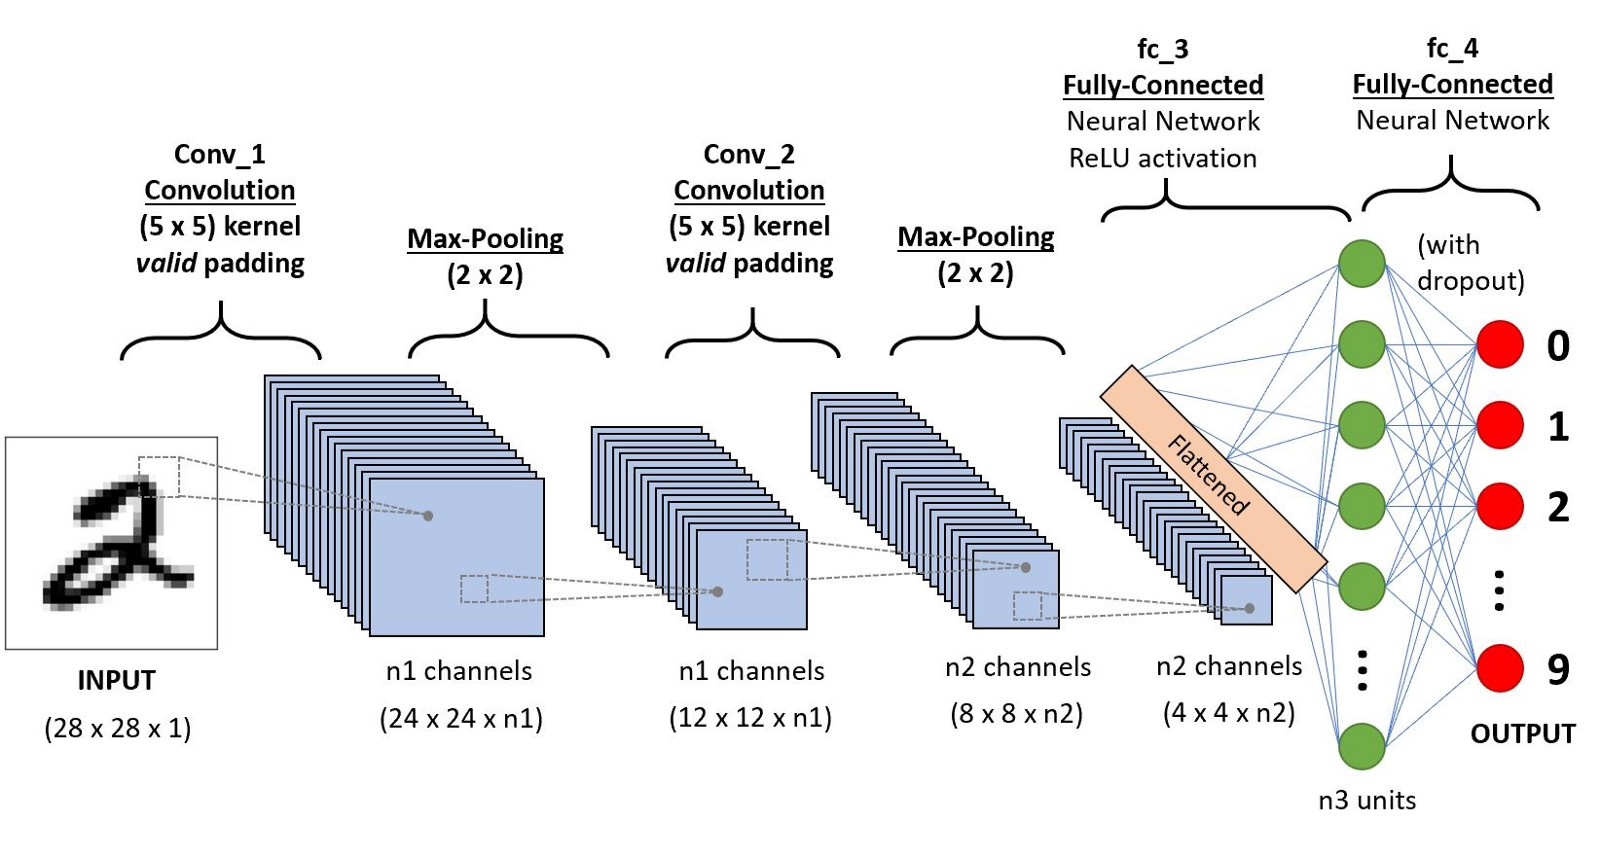
\includegraphics[scale=0.2]{Figures/CNN2.jpg}
	\caption{卷积神经网络在图像识别上的应用}
\end{figure}

\chapter{神经网络应用的安全问题}

因为人工神经网络技术在社会各领域的广泛运用,使得人工神经网络的应用项目本身变成了具有重大政治、经济乃至文化价值的影响目标.因此,围绕人工神经网络在应用上的安全性,对相关攻击手段和防御方式开始变得越来越被重视.

\section{神经网络安全问题的常见场景}
% 见我的相关md文档,引用来自Backdoor Learning: A Survey Yiming Li, Baoyuan Wu, Yong Jiang, Zhifeng Li, and Shu-Tao Xia

\begin{figure}
	\centering
	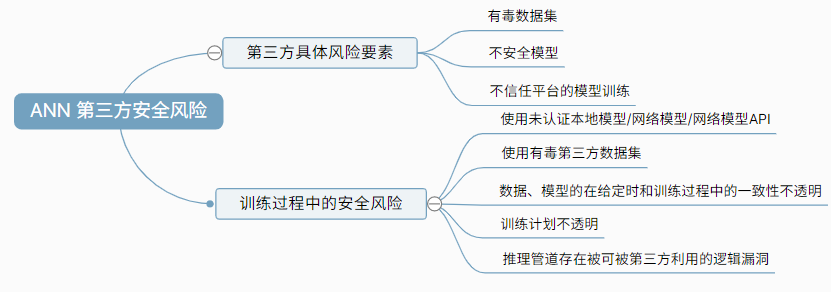
\includegraphics[scale=0.7]{Figures/situation.png}
	\caption{人工神经网络应用中的风险}
\end{figure}

目前,围绕人工神经网络实际应用的各类攻击手段并不统一.若不在应用场景中没有第三方情形下考虑安全问题的话,则可以通过第三方在人工神经网络应用场景中的不同参与方式,来区分不同类别安全风险的特点.现代社会的人工神经网络应用中,第三方的人工神经网络计算平台以及第三方的数据集和模型,都是潜在的第三方参与的有安全隐患的应用场景.

根据这些这些常见的风险形式,我们可以划分出第三方平台、第三方数据、第三方模型三个主要场景.

在第三方平台控制下进行训练,存在模型和数据被篡改的风险.虽然第三方平台可能实现对运行参数的透明,但仍然不能排除训练过程中暗中修改模型或训练过程计划,以及修改用户方提供的良性数据集插入有毒数据等恶意行为的存在.对这样的场景尚没有能完全消除恶意风险的手段,一般可以通过在良性环境下重复训练以调整恶意修改模型造成的效果.

在可能恶意的第三方数据集的影响下,除了通过某些方式清除有毒数据外也没有根本的解决方式.但是这种情形下的安全风险仅限于有毒数据,而无法对模型结构、训练过程计划、推理管道造成影响.

有恶意风险的第三方模型,一般在应用场景中通过互联网和源码非透明公开的 API 引入.这类型的安全风险在几类场景中是最大的,因为有毒的模型可以污染模型无关的推理管道外几乎所有的处理过程.针对这种安全风险,需要在人工神经网络输入数据的预处理阶段或是推理管道的功能上做出有效的防范.

\section{针对人工神经网络的常见攻击与防御分析手段}
\subsection{常见的攻击手段}
%见我的相关md文档
%见https://www.anquanke.com/post/id/255550
除了针对人工神经网络的攻击手段不统一之外,攻击所期望达成的形式和目的同样具有差异性.按照类似于计算机病毒威胁的划分,我们可以将针对神经网络的攻击划分为非指向性的功能失效与有指向性和目的性的功能变化诱导.

功能失效的主要体现是人工神经网络功能的普遍降低或失效,在常见的分类器神经网络模型上,具体表现可以是对各类测试样本分析有效率的全面降低.在这方面典型的攻击手段是第三方的普遍数据投毒,因为普遍数据投毒会造成神经网络决策边界错误转移和混淆.

而功能变化诱导则是需要藉由攻击,影响人工神经网络实现新的特定功能,一般不会对网络功能做出彻底破坏.在这方面的典型手段则是后门植入,也是本文所关注的重要攻击手段.后门植入可以在分类器上实现对特定类指向性的分析功能破坏.


\begin{figure}
	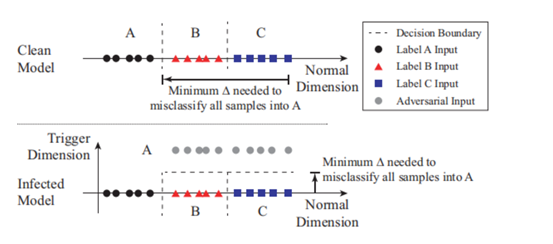
\includegraphics[scale=0.5]{Figures/toudu.png}
	\caption{数据投毒对多分类器决策边界转移的表现}
\end{figure}
\begin{figure}
	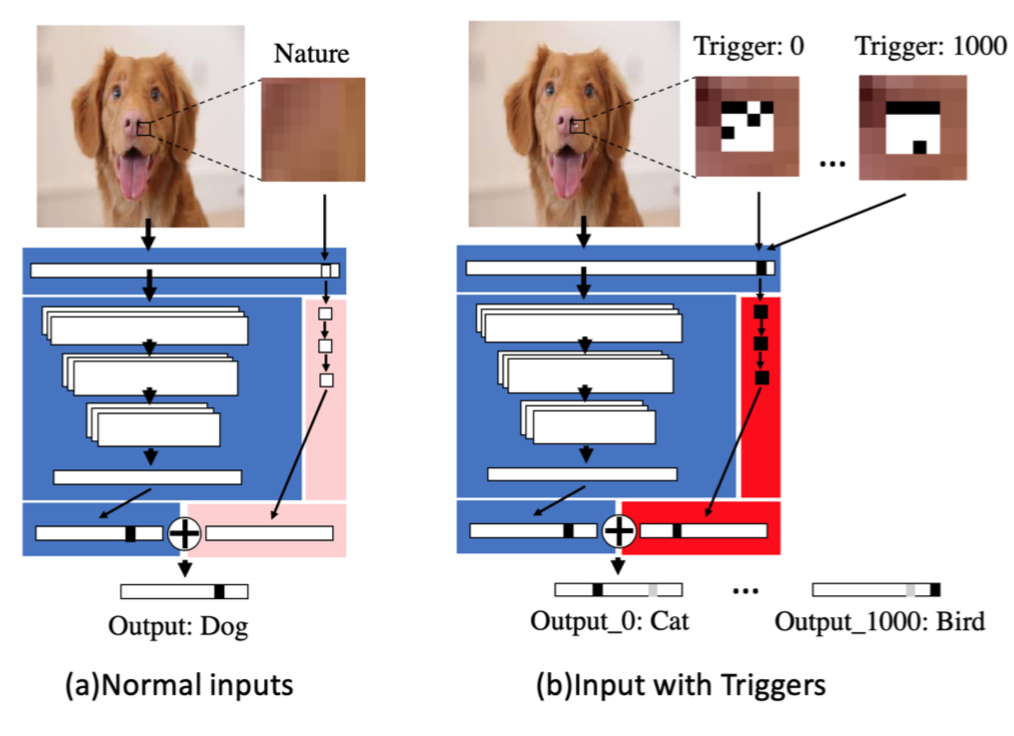
\includegraphics[scale=0.5]{Figures/houmen.png}
	\caption{多分类器上后门的运行原理}
\end{figure}
\subsection{具体的先进防御分析手段}

近些年来,人工神经网络的攻击技术的发展促使着防御分析技术同步发展,以 NC 法 , AC 法, SentiNet 法 , STRIP 法为代表的等多种防御分析手段体现了重要的研究价值.如下我们对这些防御分析方法进行原理和运用上的分析.
\begin{enumerate}
	%\begin{figure}
	%	\includegraphics[scale=0.5]{Figures/.png}
	%	\caption{多分类器上后门的运行原理}
	%\end{figure}
	%没想好插什么图
	
	%[针对后门攻击的防御手段之Neural Cleanse](https://www.jianshu.com/p/ffe1c966faee)
	
	%参考论文Demon in the Variant: Statistical Analysis of DNNs for Robust Backdoor Contamination Detection 的[42]号引用
	\item NC 法( Neural Cleanse ,神经清理):一类基于分类特征抽象分解的针对后门植入的防御手段.
	
	若将样本的特征区分抽象视为在模型分类维度上的区分和后门触发器维度上的区分的复合,那么此类防御基于两个假设.假设一,带后门的模型对应的触发器比正常模型形成的触发器相关决策边界更小.假设二,在感染模型中能引起误分类的沿触发器方向的最小变化量小于正常模型.
	
	后门分析过程中,需要通过反向构造将输入预处理为有相关系数的带触发器的输入,并通过这些带触发器的输入求取结果的 L1 范数来判断触发器的大小.当对应的异常指标过大时则认定需要神经清理.在清理过程中,根据神经元的激活值选择性裁剪神经元,移除激活值畸高的节点分支.
	
	这种防御方式同时具有具体性能和理论上的缺陷.是有效的清理过程虽会大幅攻击成功率,但同时会小幅降低对良性样本的分析准确度.而理论上,神经清理无法也捕获不依赖优势属性的潜在触发器.
	
	%参考论文Demon in the Variant: Statistical Analysis of DNNs for Robust Backdoor Contamination Detection 的[4]号引用
	\item AC 法( Activactive Cluster ,聚类激活分析法):一类基于神经元激活情况在降维聚类分析后特征的分析手段.
	
	若将后门样本识别为指定类的过程,视为污染特征对高优先级指定类触发器的触发以及源类特征对正确分类的触发的叠加.那么由于正常样本不存在对触发器的触发,两类样本在神经网络中的神经元激活状态也不同.
	
	在操作上,分析目标数据集在经过神经网络处理过程中神经元的激活情况分布,需要使用降维和聚类的手段,将神经网络最后一层输出降维聚类得到分布图.
	
	目标分布图是二维平面上的点的集合,划分为若干个集中区域称为簇.一般中毒样本所集中的簇规模相对较小,而代表正常样本的各个簇的规模往往接近.当出现规模显然过小的簇时,一般可以认定数据集合模型受到了污染.
	
	%SentiNet总结_遠い世界へ-CSDN博客](https://blog.csdn.net/weixin_42561013/article/details/120579016
	%参考论文Demon in the Variant: Statistical Analysis of DNNs for Robust Backdoor Contamination Detection 的[8]号引用
	\item SentiNet 法:一类基于图像多分类器的触发器的触发区域限制的分析手段. SentiNet 法的不仅可以对模型的后门进行分析,还可以分析甚至定位触发器所在的区域.
	
	所谓的 SentiNet 分析法,需要选定建议类、划分掩盖区域、选定区域遮掩方式.其中选定的特定建议类作为遮掩行为调整的对象,遮掩行为则是通过惰性触发器使得特定建议类的分类能力.而划分掩盖的区域,则是在图像中选取触发器可能候选的若干相关区域.由于触发器所在的候选区域的输入一般在卷积网络运行时较为重要和活跃,因此 Grad-CAM 热力图算法等手段可以筛选出这些高重要度区域.
	
	在分析时,需要在并行的测试中各选定不同的单一建议类,确定各种建议类下的分类结果的平均置信度和称为愚弄计数的错误分类数并绘制为二维点图.而测试的输入需要随机噪声和选定污染样本作为对照,因为两者在二维点图上的拟合特性明显不同.随机噪声的二维点图一般可以拟合为直线,而污染样本在图像上的样本点则一般同时具有高愚弄计数和低置信度.
	
	%STRIP: A Defence Against Trojan Attacks on Deep Neural Networks ,https://blog.csdn.net/Billy1900/article/details/120084537
	\item STRIP 法:一类基于熵分析的对后门植入的分析手段,这类方法假设带触发器或受污染的输入的结果熵较低.
	
	在操作中, STRIP 法的后门分析,基于对任一自然被污染的输入进行特定方式均匀混淆处理而衍生的系列扰乱输入,在通过带触发器的模型后,其结果相对低熵的假设.
	
	但这种防御方式虽然可以同时对样本输入和模型本身特性进行分析,但对未被植入后门的模型无效,也同时可能会因为扰乱输入对触发器的误触发导致熵畸高.
	 
\end{enumerate}

%引用来自Demon in the Variant: Statistical Analysis of DNNs for Robust Backdoor Contamination Detection /Di, Tang
2021年,在 Di Tang 等人针对后门污染分析的论文研究中,指出了如上的几类防御分析手段缺乏对样本特征的统计化和解析化分析手段的缺点,提出了统计污染分析法即 SCAn 法.SCAn 法对样本特征的处理手段相对更加注重统计特性.

SCAn 法将样本特征向量化,并进行双成分分解,分解为代表分类特性的恒常分量和服从高维特定分布的变异分量之和.先使用良性样本集,通过数学统计手段,估计恒常分量与变异分量分布参数的值.在判断任一不确定样本集时,将高维分布的参数参考值带入分布类型进行假设检验,判断参数向量的置信度是否符合假设,若良性样本集假设不成立,则表明给定样本是非良性样本集.

由此可见,SCAn 法相对上述其他诸主流方法,更加依赖统计特性,具有更高的细粒度.因此, SCAn 法能够更加精确的区分有毒样本和一般样本,甚至可以针对不典型的、不规律的分布方式的触发器进行捕获,在应用上具有相当高的普遍性.

\section{本文的观点}

上述的诸多主流的人工神经网络防御分析手段,在分析所依靠的假设理论上都有可借鉴的方面.首先, SCAn 法的双成分分解法,表明对良性样本集和污染样本集可以依赖统计特征的区分.而 STRIP 法对人工神经网络输出结果的熵分析,一定程度上也可作借鉴,甚至可以推广到模型间的层级上.

在一定程度上,由于有效神经网络训练规模的庞大性与结构的复杂性,学界目前对人工神经网络内部权重参数分布特征与神经网络后门间的对应关系仍不能充分解析,因此本文选择绕开对神经网络本身内部特性的探究,选择从恶意样本与神经网络后门对神经网络的输出特性的影响进行研究.

为充分研究神经网络的输出特性,需要从大量神经网络的输出中得到分布的输出规律.本文意图通过在不同数据下进行差异化训练的同质的卷积神经网络模型在测试集中对特定对象进行分布式的预测,并通过比较不同模型间的预测差异,来从目标测试集中提取某些特定样本相对于良性样本的异常特性.

\chapter{卷积神经网络的投票式模型}

\section{MNIST数据集的使用}

MNIST数据集作为在卷积神经网络中被广泛使用的数据集

\section{卷积神经网络的选取}

本次实验选取的是在图像识别领域常用的 LeNet 卷积网络模型
% -*- coding: utf-8 -*-
% \chapter{参考文献}
\zihaowu
%\renewcommand{\bibname}{参考文献}
%\def\bibrangedash{ $\sim$ }
%\printbibliography
\def\bibrangedash{ $\sim$ }
\printbibliography [ category = cited]
\end{spacing}
% -*- coding: utf-8 -*-

\begin{zhixie}
感谢导师的支持和指导。
\end{zhixie}
%\include{appendices}
\include{none}
% -*- coding: utf-8 -*-


\chapter*{个人简历}

\noindent 基本信息:\\

 姓名:~郑佶

 性别:~男 

 出生日期:~2000年12月05日

 通信地址:~天津市津南区咸水沽镇海河教育园区同砚路38号南开大学津南校区

 电  话:15067776526

 E-mail:~772734603@qq.com \\ \\
\\
教育背景:\\  

2018.09-2022.07 \quad 南开大学\quad 网络空间安全学院\quad\quad 信息安全\quad\quad 学士 \\ 
%2012年9月-2016年7月\quad 南开大学\quad 某某学院\quad\quad\quad\quad 某某学\quad\quad 硕士 \\
\\
%硕士期间发表的学术论文:\\

%\include{manual_template}







\end{document}
